%%%%%%%%%%%%%%%%%%%%%%%%%%%%%%%%%%%%%%%%%
% Beamer Presentation
% LaTeX Template
% Version 1.0 (10/11/12)
%
% This template has been downloaded from:
% http://www.LaTeXTemplates.com
%
% License:
% CC BY-NC-SA 3.0 (http://creativecommons.org/licenses/by-nc-sa/3.0/)
%
%%%%%%%%%%%%%%%%%%%%%%%%%%%%%%%%%%%%%%%%%

%----------------------------------------------------------------------------------------
%	PACKAGES AND THEMES
%----------------------------------------------------------------------------------------

\documentclass[10pt]{beamer}

\mode<presentation> {
	
	% The Beamer class comes with a number of default slide themes
	% which change the colors and layouts of slides. Below this is a list
	% of all the themes, uncomment each in turn to see what they look like.
	
	%\usetheme{default}
	%\usetheme{AnnArbor}
	%\usetheme{Antibes}
	%\usetheme{Bergen}
	%\usetheme{Berkeley}
	%\usetheme{Berlin}
	%\usetheme{Boadilla}
	%\usetheme{CambridgeUS}
	%\usetheme{Copenhagen}
	%\usetheme{Darmstadt}
	%\usetheme{Dresden}
	%\usetheme{Frankfurt}
	%\usetheme{Goettingen}
	%\usetheme{Hannover}
	%\usetheme{Ilmenau}
	%\usetheme{JuanLesPins}
	%\usetheme{Luebeck}
	\usepackage{tikz-qtree}
	\usepackage{latexsym}
	%\usetheme{Madrid}
	\usepackage{comment}
	\usepackage{graphicx}
	\tikzstyle{blackcircle}= [circle, draw=black, fill=black!30]
	\tikzstyle{arrow} = [thick,->,>=stealth]
	\usepackage{tikzsymbols}
	\usepackage{pgfplots}
	\pgfplotsset{compat=1.15}
	\usepackage{mathrsfs}
	\usetikzlibrary{arrows}
	\usepackage{graphicx}
	\newcommand{\F}{\mathbb{F}_2}
	\newcommand{\Cl}{\text{Cl}}
	\newcommand{\Acl}{\hat{\text{\Cl}}}
	%\usetheme{Malmoe}
	%\usetheme{Marburg}
	%\usetheme{Montpellier}
	%\usetheme{PaloAlto}
	%\usetheme{Pittsburgh}
	%\usetheme{Rochester}
	%\usetheme{Singapore}
	%\usetheme{Szeged}
	\usetheme{Warsaw}
	
	% As well as themes, the Beamer class has a number of color themes
	% for any slide theme. Uncomment each of these in turn to see how it
	% changes the colors of your current slide theme.
	
	%\usecolortheme{albatross}
	%\usecolortheme{beaver}
	%\usecolortheme{beetle}
	%\usecolortheme{crane}
	%\usecolortheme{dolphin}
	%\usecolortheme{dove}
	%\usecolortheme{fly}
	%\usecolortheme{lily}
	%\usecolortheme{orchid}
	%\usecolortheme{rose}
	%\usecolortheme{seagull}
	%\usecolortheme{seahorse}
	%\usecolortheme{whale}
	%\usecolortheme{wolverine}
	
	%\setbeamertemplate{footline} % To remove the footer line in all slides uncomment this line
	\setbeamertemplate{footline}[frame number]
	
	\setbeamertemplate{navigation symbols}{} % To remove the navigation symbols from the bottom of all slides uncomment this line
}

\usepackage{graphicx} % Allows including images
\usepackage{booktabs} % Allows the use of \toprule, \midrule and \bottomrule in tables
%\usepackage {tikz}
\newcommand{\Deg}{\text{deg}}
\usepackage{xcolor}
\usepackage{tkz-graph}
\usepackage{circuitikz}

\usepackage{physics}
\usepackage{amssymb,forest}
\usetikzlibrary{arrows.meta}

\newcommand{\mc}[2]{\multicolumn{#1}{c}{#2}}
\definecolor{Gray}{gray}{0.85}
\definecolor{LightCyan}{rgb}{0.88,1,1}


\newcommand{\cb}{\{\pm 1 \}}
\newcommand{\prob}{\text{prob}}

%-----------------------------------
%----------------------------------------------------------------------------------------
%	TITLE PAGE
%----------------------------------------------------------------------------------------

\title[Quantum--Classical Equivalence]{Quantum--Classical Equivalence for AND Functions \\[-0.1em] \small{CCC 2026}} % The short title appears at the bottom of every slide, the full title is only on the title page

\author[Bhattacharya et al.]{%
	\setlength{\tabcolsep}{1.5pt}%
	\begin{tabular}{@{}ccccc@{}}
		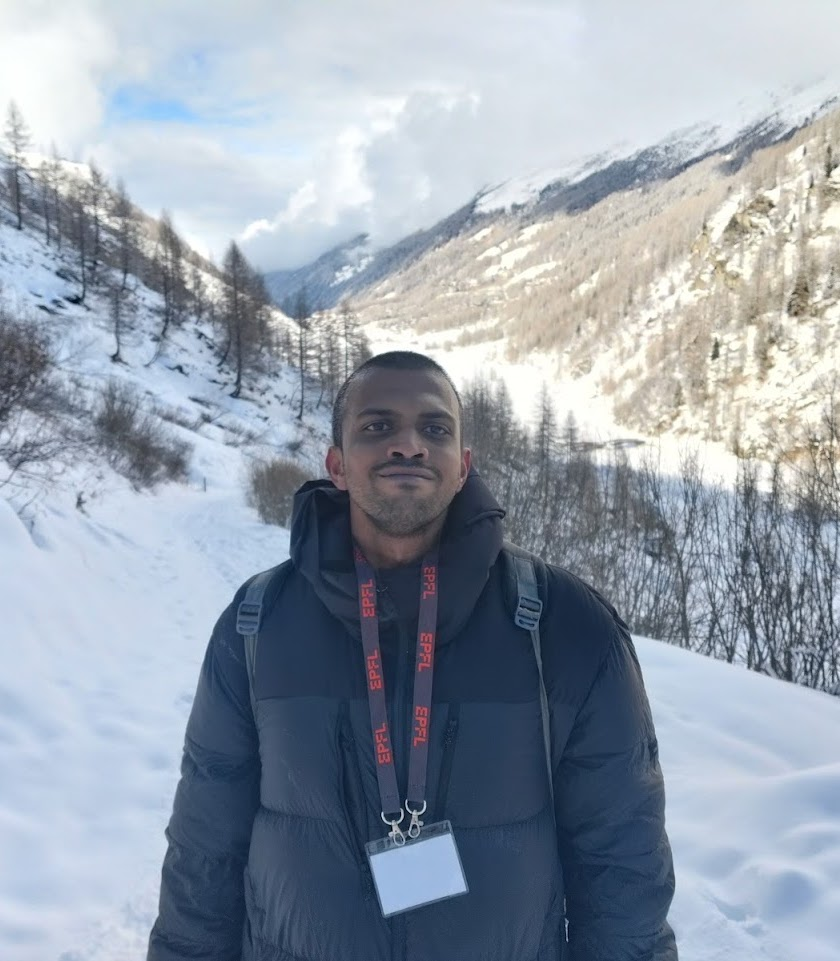
\includegraphics[width=0.17\textwidth,height=1.75cm,keepaspectratio]{sreejata_bhattacharya.jpg} &
		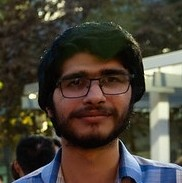
\includegraphics[width=0.17\textwidth,height=1.75cm,keepaspectratio]{farzan_byramji.jpg} &
		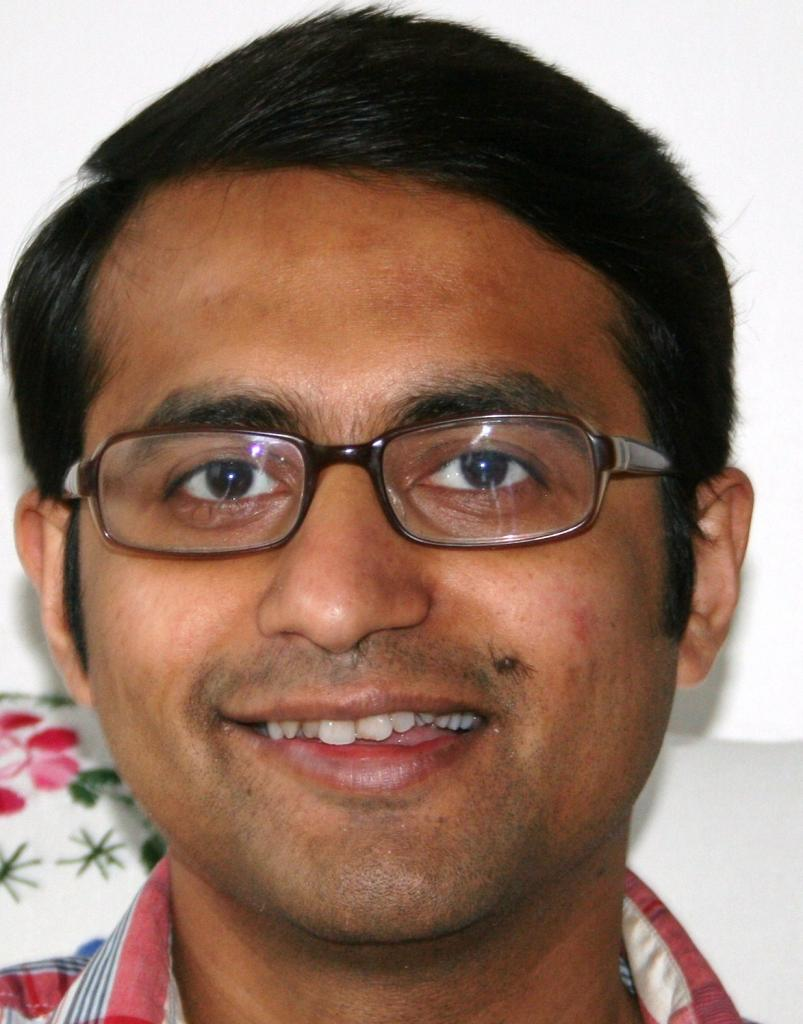
\includegraphics[width=0.17\textwidth,height=1.75cm,keepaspectratio]{arkadev_chattopadhyay.jpg} &
		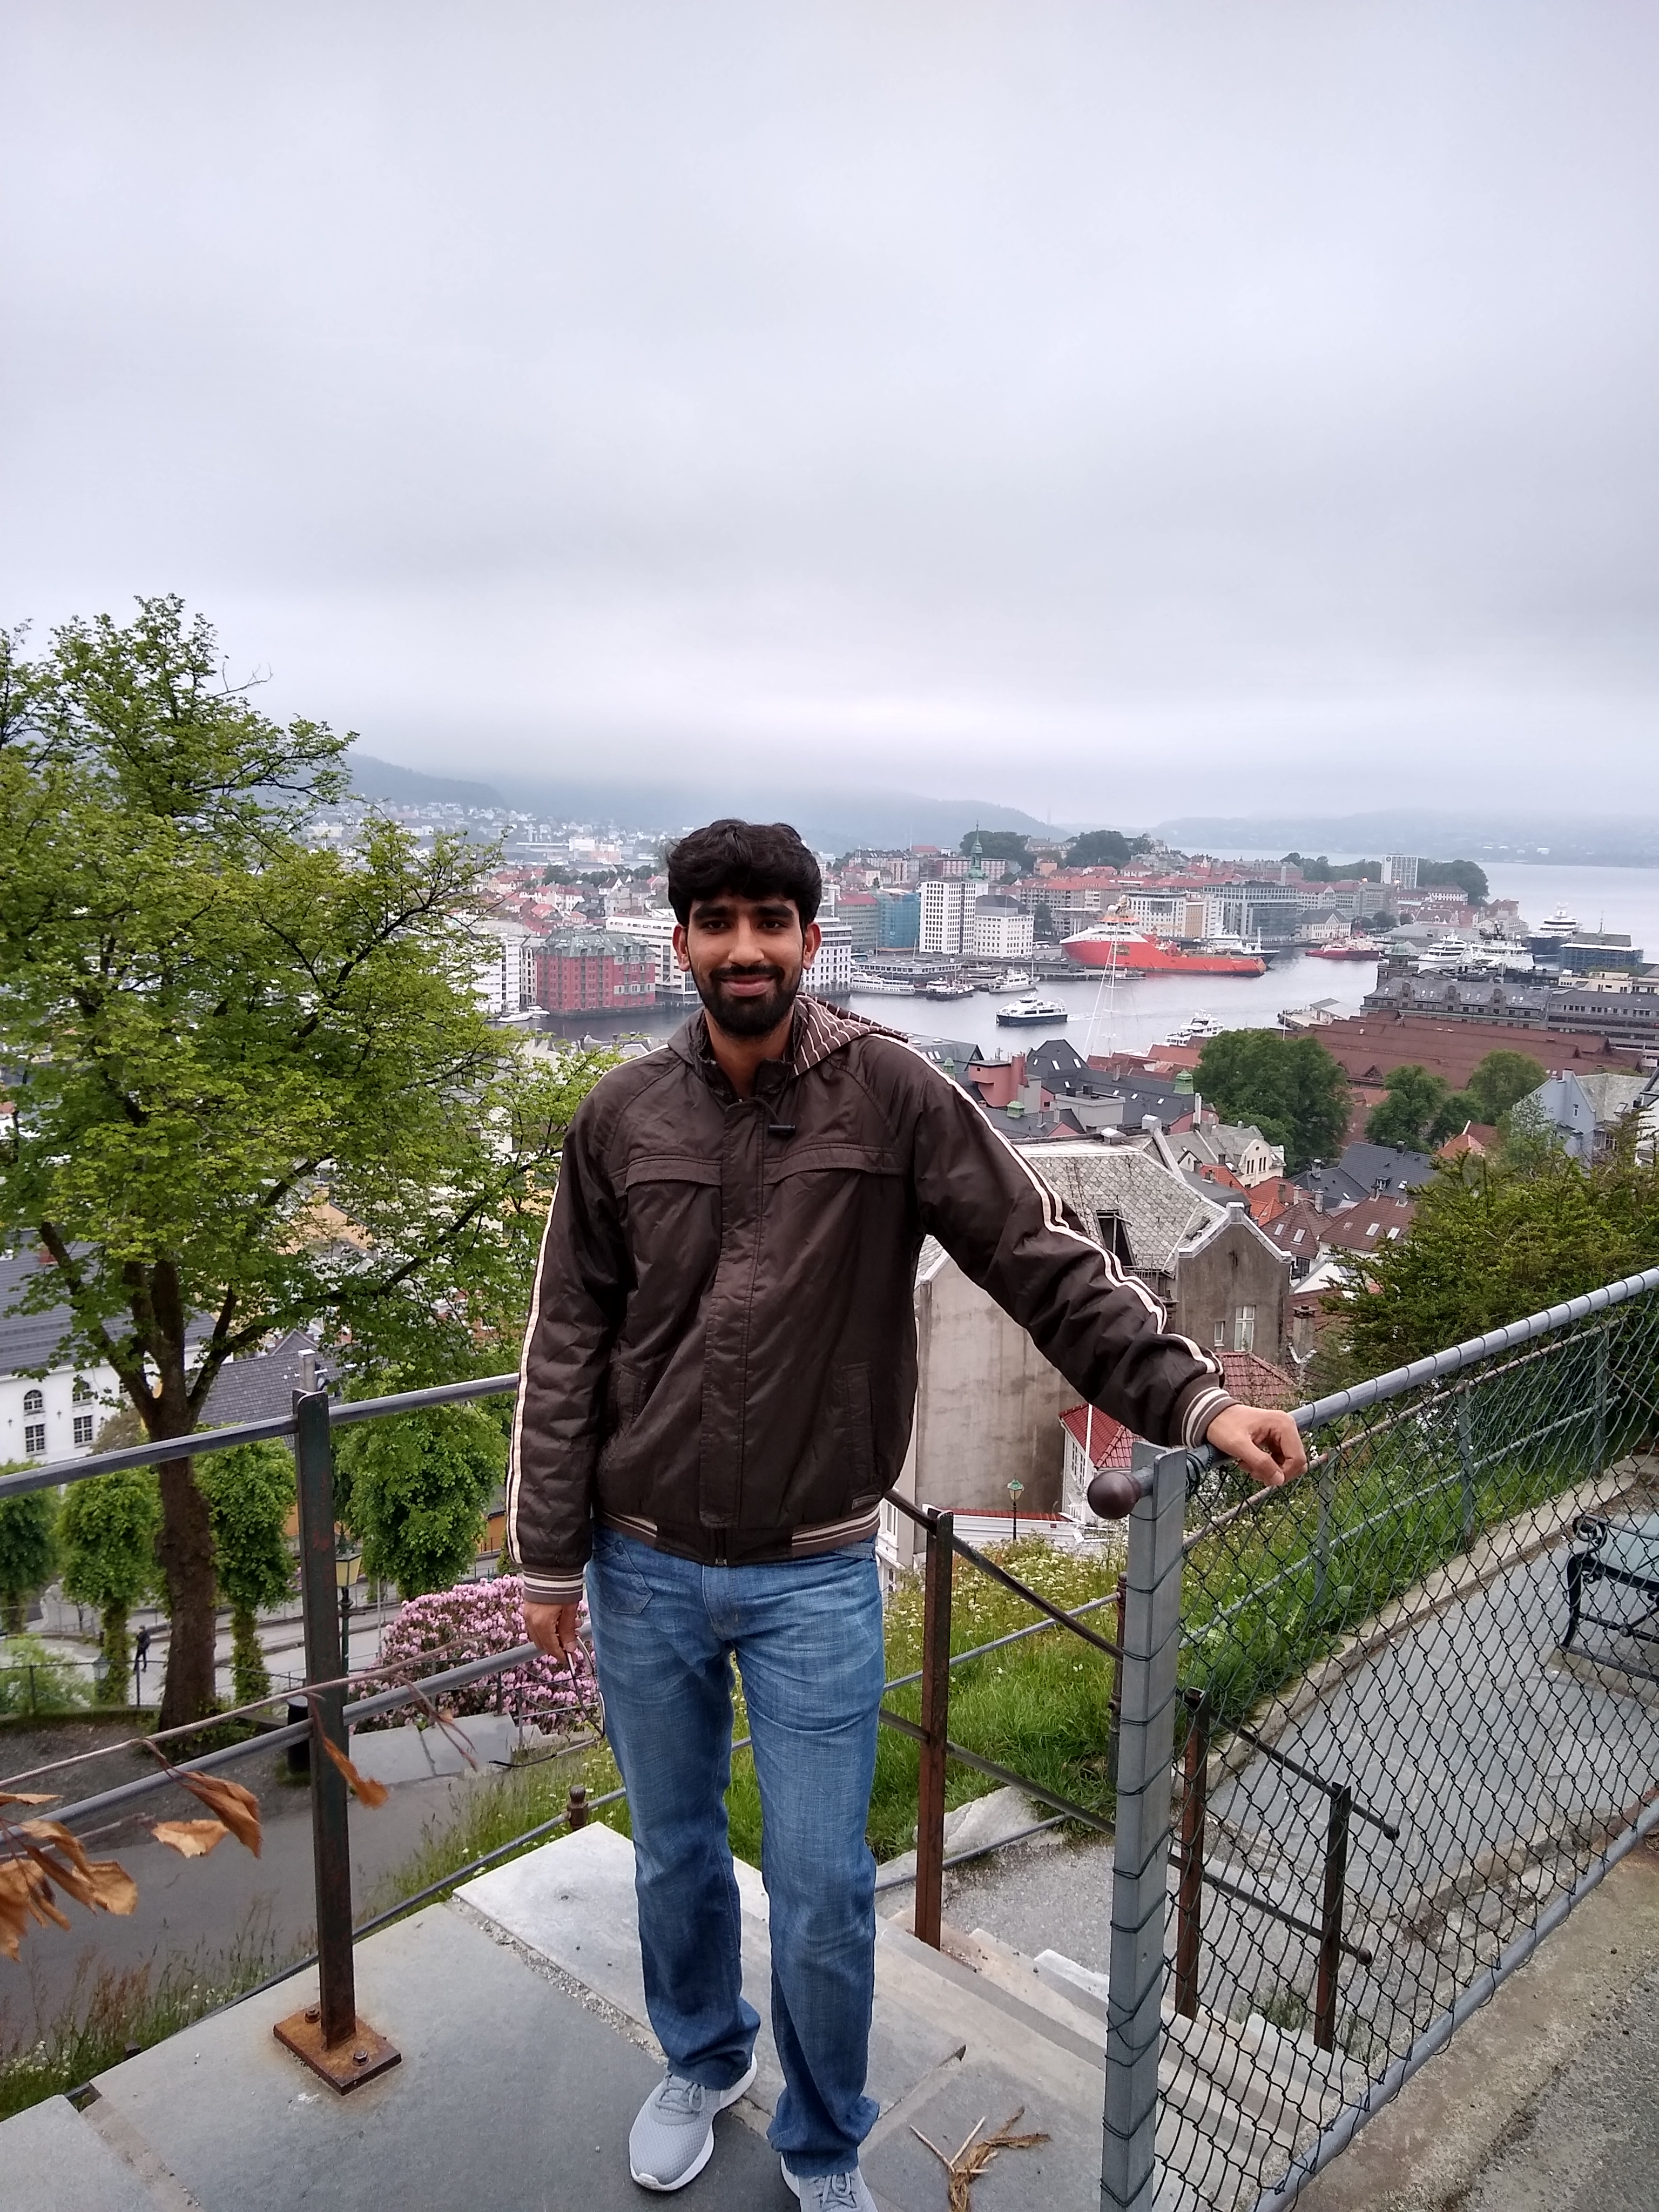
\includegraphics[width=0.17\textwidth,height=1.75cm,keepaspectratio]{yogesh_dahiya.jpg} &
		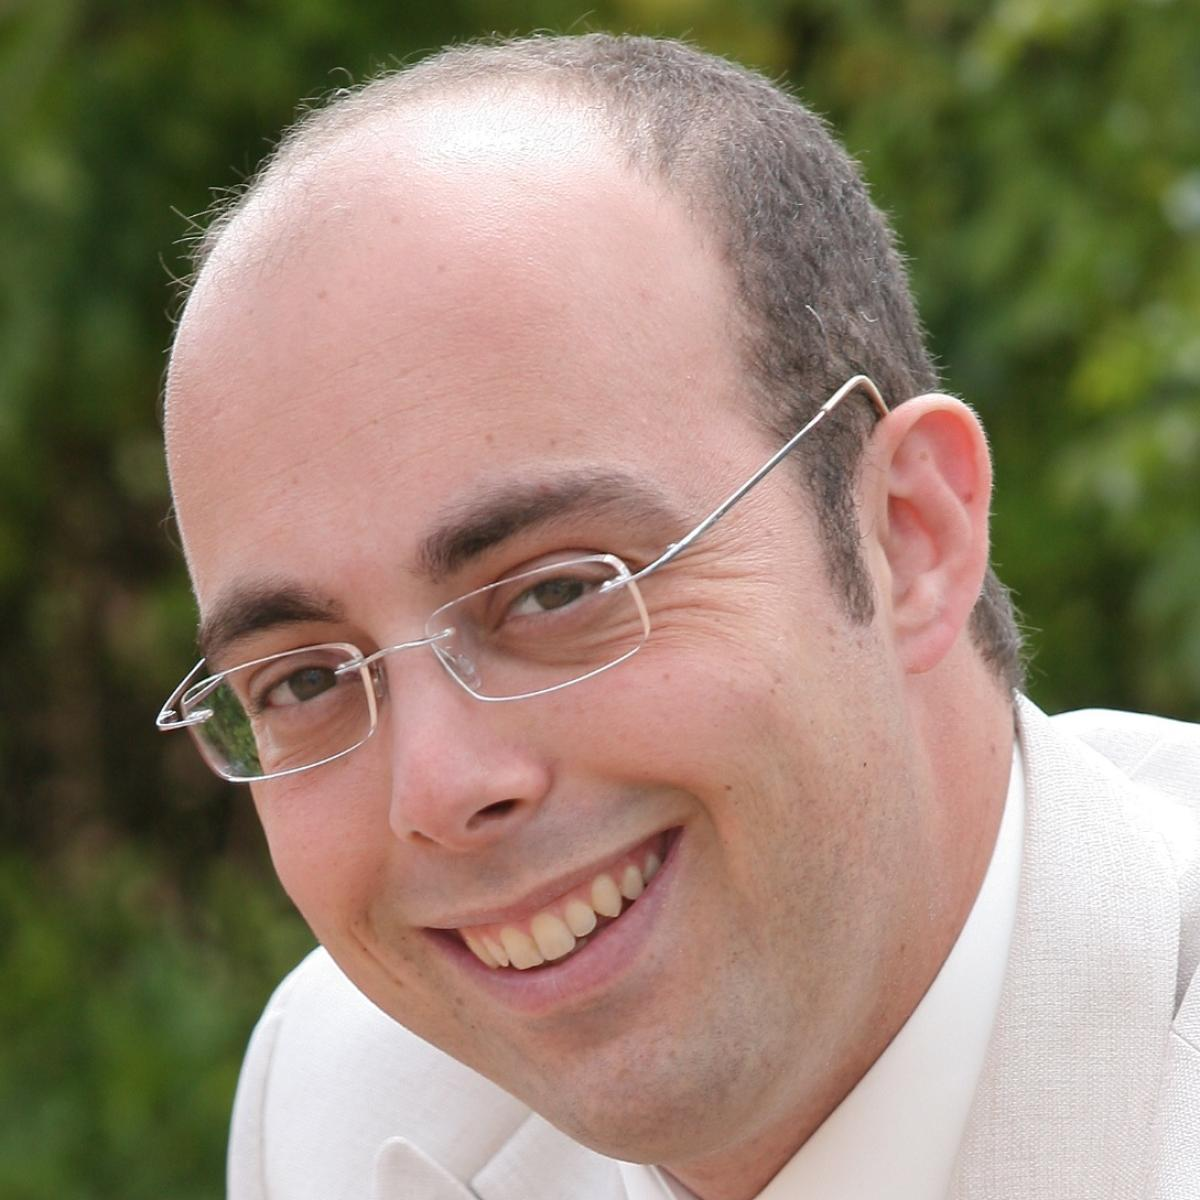
\includegraphics[width=0.17\textwidth,height=1.75cm,keepaspectratio]{shachar_lovett.jpg}
		\\[0.2em]
		\parbox[t]{0.17\textwidth}{\centering\tiny\textcolor{blue}{Sreejata Kishor\\Bhattacharya (TIFR)}} &
		\parbox[t]{0.17\textwidth}{\centering\tiny Farzan Byramji (UCSD)} &
		\parbox[t]{0.17\textwidth}{\centering\tiny Arkadev\\Chattopadhyay (TIFR)} &
		\parbox[t]{0.17\textwidth}{\centering\tiny Yogesh Dahiya (UCSD)} &
		\parbox[t]{0.17\textwidth}{\centering\tiny Shachar Lovett (UCSD)}
	\end{tabular}%
}
\institute[TIFR] % Your institution as it will appear on the bottom of every slide, may be shorthand to save space
{

	
}
%\date{\today} % Date, can be changed to a custom date
\date{ }
\begin{document}
	
	\begin{frame}
		\titlepage % Print the title page as the first slide
	\end{frame}
	
	
	
	%----------------------------------------------------------------------------------------
	%	PRESENTATION SLIDES
	%----------------------------------------------------------------------------------------
	
	%------------------------------------------------
	\newcommand{\cube}{\{\pm 1\}}
	\section{Introduction}

\begin{frame}{introducing quantum communication}
Our model of quantum communication: Alice and Bob share an unlimited number of EPR pairs; have their own auxiliary quantum systems, and can communicate classical bits \footnote{Therefore they can do quantum teleportation.}. Cost of the communication protocol is the number of classical bits communicated. 

\begin{figure}[htbp]
	\centering % Centers the image
	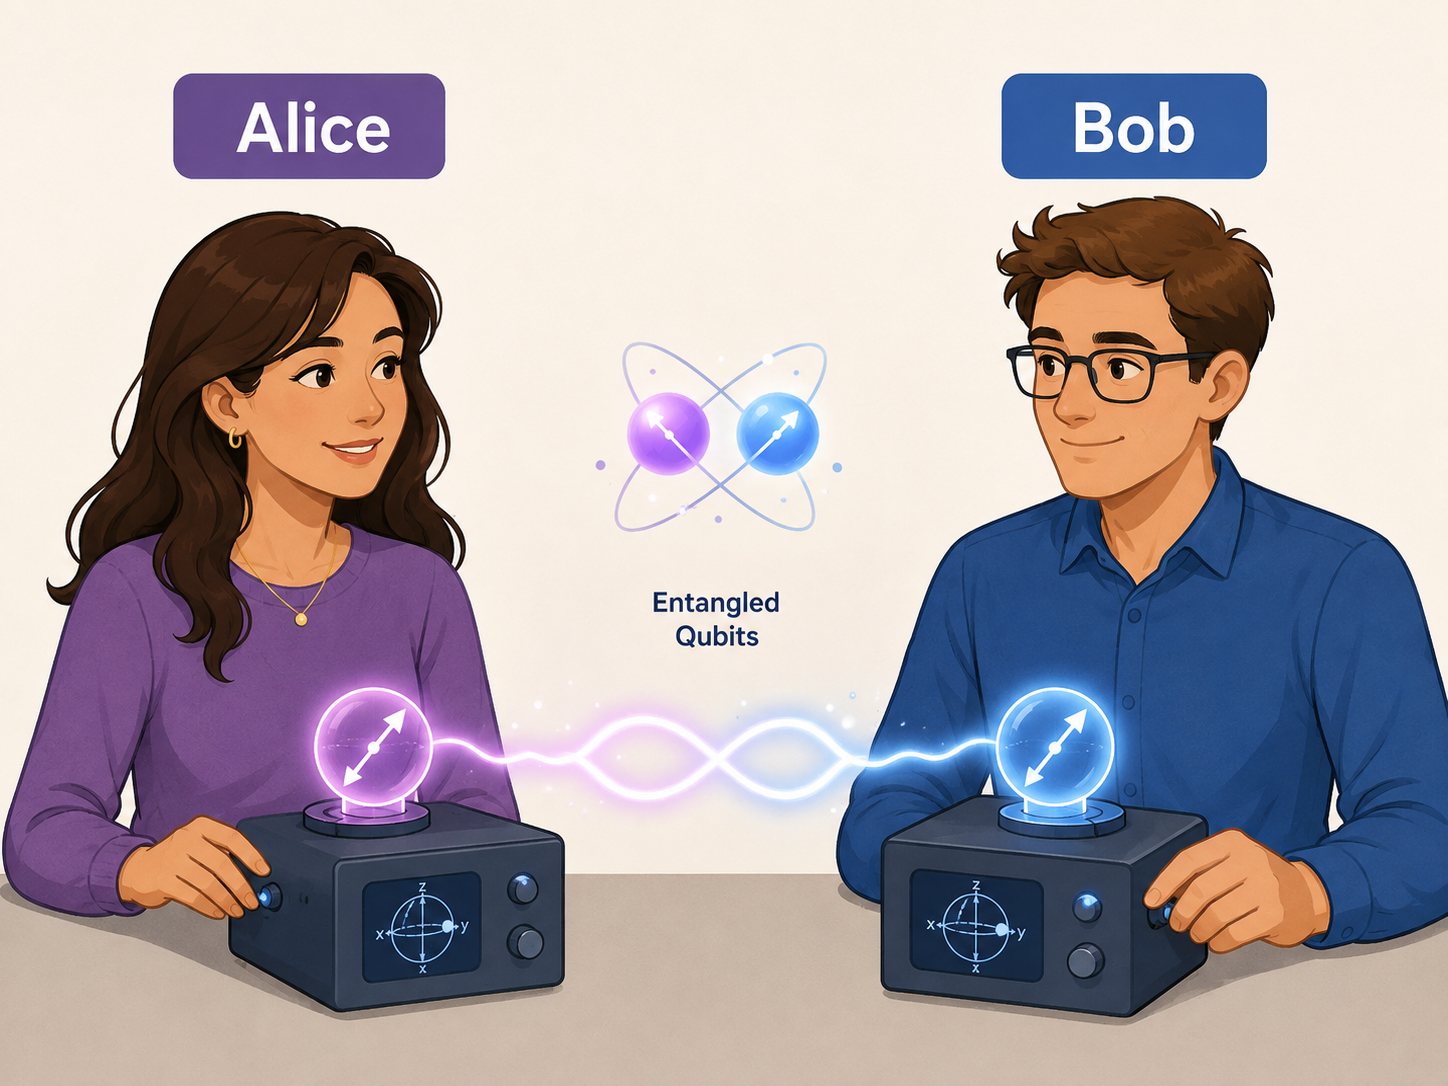
\includegraphics[width=0.7\textwidth]{quantum_communication.png} % Loads the image
	\caption{This is the caption for my image.}
	\label{fig:my_image} % Label used for cross-referencing
\end{figure}


\end{frame}	


\begin{frame}
	\textcolor{red}{\textbf{Quantum-Equivalence Conjecture}}: For a total function $f: \{0,1\}^n  \rightarrow \{0,1\}$, 
	$$R(f) \leq \text{poly}(Q(f))$$
	where
	\begin{itemize}
		\item $R(f)=$ classical randomized communication complexity
		\item $Q(f)=$ quantum communication complexity (with prior entanglement)
	\end{itemize}
	
	\textbf{Major open problem in communication complexity. First formally proposed by Shi and Zhu (2008)}
	
	
	
\end{frame}

\begin{frame}
	\textcolor{red}{\textbf{Our result}}: For AND functions, $f= g \circ \text{AND}_2$,
	$$ D(f) \leq \text{poly}(Q(f), \log(n)$$
	where $D(f)=$ classical deterministic communication complexity. \newline
	Thus, Quantum Equivalence Conjecture is true for AND functions up to $\text{polylog}(n)$ factors. \newline
	
	This answers an open problem of Razborov [2002].
	
	
	
\end{frame}

\begin{frame}
	
	\textbf{Why study AND functions?}
	\begin{itemize}
		\item<1-> Lifted functions form a large class of interesting communication problems. They form a testbed for all major conjectures in communication complexity (e.g, Log Rank Conjecture, Log Approximate Rank Conjecture [now known to be false], Quantum Equivalence Conjecture)
		\item<2-> Of particular interest is the case when the lifting gadget is as simple as possible, i.e., it has only two bits. In this case, the gadget does not have too much ability to obfuscate the inputs between Alice and Bob.
		\item<3-> There are only two nontrivial gadgets on 2 bits: XOR and AND. Both XOR and AND functions have been extensively studied in the literature.
	\end{itemize}
	
\end{frame}



\begin{frame}
	
	\textbf{AND functions}
	\begin{itemize}
		\item<1-> There is a base function $g: \{0,1\}^n \rightarrow \{0,1\}$. Alice has an input $x \in \{0,1\}^n$, Bob has an input $y \in \{0,1\}^n$. Their goal is to compute
		$$g(x_1 \land y_1, \cdots  , x_n \land y_n)$$
	\end{itemize}
	
\end{frame}



\begin{frame}{Prior work}
	\begin{itemize}
		\item<1-> \textbf{Razborov (2002)} proved the Equivalence conjecture for functions of the form $g \circ \text{AND}_2$, where $g$ is a symmetric function. 
		\item<2-> An easy adaptation of the same argument proves the results for functions of the form $g \circ h$, where $h$ is any gadget inside whose truth table both AND and OR can be embedded.
		\item<3-> \textbf{Burhman and deWolf (2003)} noticed a relation between $Q(g \circ \text{AND}_2)$ and various complexity measures of $g$, and conjectured a particular relation between them (to be described in detail soon).
		\item<4->\textbf{Kremer (1996)} proved log-approximate rank lower bounds quantum communication complexity.
		\item<5-> \textbf{Lovett, Knop, McGuire, Yuan (2021)} proved the log rank conjecture for AND functions. By an intermediate result in their proof, it became  clear that proving the relation conjectured by Burhman and deWolf would also imply the Quantum Equivalence Conjecture for $\text{AND}$ functions.
	\end{itemize}
	
\end{frame}



\begin{frame}{Prior work}
	\begin{itemize}
		\item<1-> \textbf{Chattopadhyay, Dahiya, Lovett (2026)} proved that de-Morgan sparsity and approximate de-Morgan sparsity are polynomially related.
		\item<2-> They also show the Quantum Equivalence Conjecture for functions of the form $g \circ \text{EQ}_4$.
		\item<3-> We extend their work to show the relation between quantities conjectured by Burhman and deWolf. This implies the Quantum-Equivalence Conjecture for AND functions.
	\end{itemize}
	
\end{frame}
	
	\section{Quantum communication complexity and other measures}
\begin{frame}{prior results}
	\begin{itemize}
		\item<1-> A result of Kremer \footnote{The result of Kremer only lower bounds clean-quantum communication complexity. [BdW01] observed that it readily implies general quantum communication lower bounds too. Another lower bound in terms of $\gamma_2$ norm was given by Lee and Shraibman [LS07]}: 
		$$Q^{cc}(F) \geq \text{poly}(\log(\text{rank}^{1/3}(F))$$
		where 
		$$ \text{rank}^{1/3}(F)= \text{inf} \{\text{rank}(G) \mid ||G-F||_{\infty} \leq 1/3\} $$
		\item<2-> Thus, log-approximate rank conjecture for a class of functions also implies quantum-equivalence conjecture for that class of functions.
		\item<3-> It is known that LARC is false in general \textbf{(Mande, Suhail, Chattopadhyay, 2019)}. Nevertheless, in this work we show LARC is true for AND functions (upto $\text{polylog}(n)$ factors); thereby also establishing the QEC for AND functions.	
	\end{itemize}
	
	
\end{frame}


\begin{frame}{prior results}
	
	
	
	\textcolor{red}{In case Yogesh has defined this properly in his previous talk I shall skip the next few slides.}
	
	\begin{itemize}
		\item<1-> Any function $g: \{0,1\}^n \rightarrow \mathbb{R}$ has a unique representation as a multilinear polynomial:
		$$ g(x) = \displaystyle \sum_{S \subseteq [n]} \alpha_S x_S$$
		where $x_S= \displaystyle \prod_{i \in S} x_i$. \newline
		
		\textbf{Note: }This is not the Fourier decomposition where the domain is $\{ \pm 1\}$. Also note that we are working over $\mathbb{R}$, not $\mathbb{F}_2$. 
	\end{itemize}
	
\end{frame}


\begin{frame}
	
	
	
	\begin{itemize}
		\item<1-> Any function $g: \{0,1\}^n \rightarrow \mathbb{R}$ has a unique representation as a multilinear polynomial:
		$$ g(x) = \displaystyle \sum_{S \subseteq [n]} \alpha_S x_S$$
		where $x_S= \displaystyle \prod_{i \in S} x_i$. \newline
		Define sparsity of $g$, $\text{spar}(g)$, to be the number of nonzero monomials in this representation. 
		
	\end{itemize}
	
\end{frame}


\begin{frame}{}
	
	
	
	\begin{itemize}
		\item<1-> The conjecture in [BdW01]:
		
		$$ \text{rank}^{1/3} [g \circ \text{AND}_2] \approx \text{spar}(g)$$
		\item<2-> Our main result:
		
		$$ \log \text{spar}(g) \leq \text{poly}\left(\log ( \text{rank}^{1/3} (g \circ \text{AND}_2), \log(n) )\right) $$ \footnote{Other direction is trivial}
		
	\end{itemize}
	
\end{frame}

\begin{frame}
	
\textbf{How this implies the Quantum Equivalence Conjecture}
	
	\begin{itemize}
		\item<1-> Recall we want to upper bound $D(f)$ in terms of $\text{log} \left( \text{rank}^{1/3} (f \circ \text{AND}_2)\right)$
		\item<2-> \textbf{Knop, Lovett, McGuire, Yuan} showed that
		$$ \log D(g \circ \text{AND}_2) \leq \text{poly}(\log \text{spar}(g), \log(n))$$
		\item<3-> Since our result upper bounds $\text{spar}(g)$ in terms of $\text{rank}^{1/3}(g \circ \text{AND}_2)$, the result immediately follows.
	\end{itemize}
	
\end{frame}





\section{Proof sketch}
\begin{frame}
\textbf{Goal: }Upper bound $\text{spar}(g)$ in terms of $\text{rank}^{1/3} (g \circ \text{AND}_2)$

\begin{itemize}
	\item<1-> Assume, for the sake of contradiction, $\text{spar}(g)$ is large and $\text{rank}^{1/3} (g \circ \text{AND}_2)$ is small.
	\item<2-> From the second assumption, we have functions
	$$ a_i, b_i : \{0,1\}^n \rightarrow [0,1] , i= 1, 2, \cdots , m$$
	and constants $\alpha_i, i = 1, 2, \cdots , m$ such that
	
	$$\left| g(x \land y) - \displaystyle \sum_{i=1}^{m} \alpha_i a_i(x) \land b_i(y)\right| \leq 1/3$$
	\item<2-> By standard techniques (eg John's lemma), we can assume $\sum |\alpha_i| \leq L$ (where $\log L \leq \text{polylog} (m)$)
\end{itemize}

\end{frame}

\begin{frame}
	\textbf{Goal: }Upper bound $\text{spar}(g)$ in terms of $\text{rank}^{1/3} (g \circ \text{AND}_2)$
	
	\begin{itemize}
		\item<1-> We shall construct a function $f$ (to be obtained from $g$) such that
		\begin{itemize}
			\item Approximate degree of $f$ is small
			\item Degree of $f$ is high
		\end{itemize}
		This contradicts known relations between degree and approximate degree (first proven by Nisan-Szegedy; constants were optimized later).
		
		\item<2-> We shall get a low-degree approximating polynomial from the inequality 
			$$\left| g(x \land y) - \displaystyle \sum_{i=1}^{m} \alpha_i a_i(x) \land b_i(y)\right| \leq 1/3$$
			whereas the high sparsity of $g$ will guarantee the original polynomial has high degree.
	\end{itemize}
	
\end{frame}


\begin{frame}
	\textbf{Goal: }Upper bound $\text{spar}(g)$ in terms of $\text{rank}^{1/3} (g \circ \text{AND}_2)$
	
	\begin{itemize}
		\item<1-> Note that every function $f: \{0,1\}^n \rightarrow \mathbb{R}$ can also be represented as a function $\tilde{f}: \{ \pm 1\}^n \rightarrow \mathbb{R}$. It is easy to see that their degrees are the same. \newline
		
		 \textbf{Convention: }For a function $f: \{0,1\}^n \rightarrow \mathbb{R}$, we denote its equivalent function with the domain $\{ \pm 1\}^n$ by $\tilde{f}: \{ \pm 1\}^n \rightarrow \mathbb{R}$.
		\item<2-> For upper-bounding the approximate degree, we shall look at functions in the $\{\pm 1\}^n$ domain. For lower bounding the degree, we shall look at functions in the $\{ 0, 1\}^n$ domain. Since the degree is invariant under change of domain, this is ok.
	\end{itemize}
	
\end{frame}

\begin{frame}
	
	\begin{itemize}
		\item \textbf{Observation: }Given the expression 
		$$ g(x \land y) \approx \displaystyle \sum_{i=1}^{m} \alpha_i a_i(x) \land b_i(y),$$
		we can hit each $a_i$ by a restriction+averaging operator $(\rho, \delta)$, replace each $b_i$ by a constant, and get an approximation for $g_{\rho}$
	\end{itemize}
\end{frame}


\begin{frame}
	
	\textbf{Restriction+averaging operators: }
	
	A \textbf{restriction+averaging operator} is denoted by a string $R \in \{0,1,*,\Delta\}^n$. It converts a function $f: \{0,1\}^n \rightarrow \mathbb{R}$ to a function $f: \{0,1\}^{\text{free}(R)} \rightarrow \mathbb{R}$ where $\text{free}(R)= \{i | R_i=*\}$. The transformation is as follows:
	\begin{itemize}
		\item If $R_i=b \in \{0,1\}$, fix the $i$-th coordinate to $b$.
		\item If $R_i= \Delta$, average over the $i$-th coordinate.
		\item If $R_i=*$, keep the $i$-th coordinate free.
	\end{itemize}
	
	We shall associate a partial assignment $\rho \in \{0,1,*\}^n$ to each restriction+averaging operator $R$: $\rho$ is obtained from $R$ by changing all the $\Delta$'s to 0's. 
	
	
\end{frame}

\begin{frame}
	\textbf{Goal: }Upper bound $\text{spar}(g)$ in terms of $\text{rank}^{1/3} (g \circ \text{AND}_2)$
	
	\begin{itemize}
		\item<1-> We shall define a distribution $\mathcal{D}$ over \textit{restriction+averaging operators} $R$ such that for any $\tilde{a}: \{ \pm 1\}^n \rightarrow [0,1]$,
		$$ \text{E}_{R \sim \mathcal{D}} [ |\tilde{a}_{R}|^{\geq d}] \leq \varepsilon$$
		
		where $|\tilde{f}|^{\geq d}$ denotes $\ell^1$ Fourier weight above level $d$
		\item<2-> ... and such that $\text{E}_{R \sim \mathcal{D}}[ f_{\rho}] \geq D$, where $\rho$ is the partial assignment associated with $R$.
	\end{itemize}	
	
\end{frame}

\begin{frame}

	\begin{itemize}
		\item<1-> The first property, along with the expression for approximate rank, will give that $\text{approx-deg}(g_{\rho}) \leq d$ for a typical $R \sim \mathcal{D}$
		\item<2-> The second property will give that $\text{deg}(g_{\rho}) \geq D$ for a typical $R \sim \mathcal{D}$.
		\item<3-> If the gap between $d$ and $D$ is large enough, we are done.
	\end{itemize}	
	
\end{frame}


\begin{frame}{Obtaining an approximation for $f_{\rho}$}
\begin{itemize}
	\item<1-> Recall the expression we got from the low-approximate rank assumption:
	$$ g(x \land y) \approx \displaystyle \sum_{i=1}^{m} \alpha_i a_i(x) b_i(y)$$
	$$ a_i, b_i: \{0,1\}^n \rightarrow [0,1]$$
	$$ \displaystyle \sum_i |\alpha_i| \leq L$$
	\item<2-> \textbf{Claim: }Given a restriction+averaging operator $R$, with $\rho$ its associated partial assignment, there exist constants $c_1, c_2, \cdots , c_m \in [0,1]$ such that
	$$ g_{\rho} (z) \approx \displaystyle \sum_{i=1}^{m} \alpha_i c_i (a_i)_{R} (z)$$

\end{itemize}	

\end{frame}

\begin{frame}{Obtaining an approximation for $f_{\rho}$}
	\begin{itemize}
		\item<1-> \textbf{Claim: }Given a restriction+averaging operator $R$, with $\rho$ its associated partial assignment, there exist constants $c_1, c_2, \cdots , c_m \in [0,1]$ such that
		$$ g_{\rho} (z) \approx \displaystyle \sum_{i=1}^{m} \alpha_i c_i (a_i)_{R} (z)$$
		\item<2-> I will show this only for the special case $R= \{\Delta , *, *, *, \cdots , *\}$. General case should be clear from this.
		\item<3-> So, $\rho = \{0, *, *, *, \cdots , *\}$.
	\end{itemize}	
	
\end{frame}


\begin{frame}{Obtaining an approximation for $f_{\rho}$}
	\begin{itemize}
		\item<1->I will show this only for the special case $R= \{\Delta , *, *, *, \cdots , *\}$. General case should be clear from this. So, $\rho = \{0, *, *, *, \cdots , *\}$.
		\item<2-> Plugging $y_0= (0, 1, 1, \cdots , 1), x= (1, z_2, z_3, \cdots , z_n)$, we get
		$$ g(0, z_2, z_3, \cdots , z_n) \approx \displaystyle \sum_{i=1}^{m} \alpha_i a_i(1, z_2, \cdots , z_n) b_i(y_0)$$
		Plugging $y_0= (0, 1, 1, \cdots , 1), x= (0, z_2, z_3, \cdots , z_n)$,
		$$ g(0, z_2, c_3, \cdots , z_n) \approx \displaystyle \sum_{i=1}^{m} \alpha_i a_i(0, z_2, z_3, \cdots , z_n) b_i(y_0) $$
		\item<3-> Average these two expressions:
		$$ g(0, z_2, \cdots , z_n) \approx \displaystyle \sum_{i=1}^{m} \alpha_i b_i(y_0) (a_i)_R(z)$$
			
	\end{itemize}	
	
\end{frame}

\begin{frame}{Exhibiting a gap between degree and approximate degree}
	\begin{itemize}
		\item<1-> \textbf{Conclusion: }If $R$ is a restriction+averaging operator and $\rho$ is the associated partial assignment, we get an approximation for $g_{\rho}$ in terms of the $(a_i)_R$'s.
		\item<2-> \textbf{Our next goal: }Using the fact that sparsity of $g$ is high, we define a distribution $\mathcal{D}$ over restriction+averaging operators $R$ such that:
		\begin{itemize}
			\item For all $a: \{0,1\}^n \rightarrow [0,1]$ ,$\text{E}_{R \sim \mathcal{D}}[\tilde{\text{deg}}(a_{R})] \leq d$ \textcolor{red}{(we will do something slightly different actually)}
			\item $\text{E}_{(R \sim \mathcal{D})} [\text{deg}(g_{\rho})] \geq D$ where $\rho$ is the partial assignment corresponding to $R$.
		\end{itemize} 
		\item<3-> If we can do this with a sufficiently big gap between $d$ and $D$, from the previous observation we get that the approximate degree of $g_{\rho}$ is very small; whereas teh second property implies the exact degree of $g_{\rho}$ is very large. But Nisan-Szegedy implies for any Boolean function, degree and approximate degree are polynomially related. Contradiction.
		
		
	\end{itemize}	
	
\end{frame}



\begin{frame}{Simplifying any bounded function}
\textbf{First requirement: }
\begin{itemize}
\item<1-> This is what we will show: \newline
For any $\tilde{a}: \{ \pm 1\}^n \rightarrow [0,1]$, 
$$ \text{E}_{R \sim \mathcal{D}} [|| \tilde{a}_R ||^{\geq d}] \leq \varepsilon$$
where $||f||^{\geq d}$ denotes total $\ell^1$ Fourier mass above level $d$. \newline
Notice that we switched to $\{ \pm 1\}$ domain here.
\item<2-> If we achieve this, the total $\ell^1$ Fourier mass above level $d$ of the function
$$ \displaystyle \sum_{i=1}^{L} \alpha_i c_i (a_i)_R$$ will be at most $L \varepsilon$, which we will set to be $<1/100$. Thus, on expectation, the approximate degree of $g_{\rho}$ will be $\leq d$.
\end{itemize}
\end{frame}

\begin{frame}{Simplifying any bounded function}
\textbf{Why switching to the $\{ \pm 1 \}$ basis is helpful:}
\begin{itemize}
	\item<1-> Let $\tilde{f}: \{ \pm 1\}^n \rightarrow \mathbb{R}$ be any function. Its Fourier expansion is
	$$ \tilde{f} = \displaystyle \sum_{S \subseteq [n]} \hat{\tilde{f}}(S) \chi_S$$
	\item<2-> Suppose we hit $\tilde{f}$ by a restriction+averaging operator $R$, which averages over some subset $T$ of variables. Then, we have
	$$ \tilde{f}_R = \displaystyle \sum_{S \cap T = \phi} \hat{\tilde{f}}(S) \chi_S$$
	\item<3->Thus, averaging out over a variable kills all monomials containing it.
\end{itemize}
\end{frame}

\begin{frame}{Defining the distribution}

\begin{itemize}
	\item<1-> Assume $g: \{0,1\}^n \rightarrow \{0,1\}$ has $\geq s$ non-zero monomials in the deMorgan basis. Let $\mathcal{F} \subseteq 2^{[n]}$ denote the set of nonzero monomials. 
	\item<2-> By \textbf{Sauer-Shelah lemma}, the VC dimension of $\mathcal{F}$ is at least $\Omega (\log(s)/\log(n))$.
	\item<3-> Let $T \subseteq [n]$ be a shattered set of size $\geq \Omega(\log(s)/\log(n))$.
	\item<4-> For any $A \subseteq T$, there exists $S \in \mathcal{F}$ such that $S \cap T = A$.
\end{itemize}

\end{frame}


\begin{frame}{Defining the distribution}
	
	\begin{itemize}
		\item<1-> Assume $g: \{0,1\}^n \rightarrow \{0,1\}$ has $\geq s$ non-zero monomials in the deMorgan basis. Let $\mathcal{F} \subseteq 2^{[n]}$ denote the set of nonzero monomials. 
		\item<2-> By \textbf{Sauer-Shelah lemma}, the VC dimension of $\mathcal{F}$ is at least $\Omega (\log(s)/\log(n))$.
		\item<3-> Let $T \subseteq [n]$ be a shattered set of size $\geq \Omega(\log(s)/\log(n))$.
		\item<4-> For any $A \subseteq T$, there exists $S \in \mathcal{F}$ such that $S \cap T = A$.
	\end{itemize}
	
\end{frame}

\begin{frame}{Defining the distribution}
	
	\begin{itemize}
		\item<1-> Let $T$ be the large shattered subset.
		\item<2-> For every $i \in T$, set 
		$$
		R(i) = \begin{cases}
			* & \text{ with probability }p \\
			\Delta & \text{ with probability }1-p
		\end{cases}
		$$
	(Here $p$ is small but non-negligible.)
	\item<3-> Let $A = \{i | i \in T, R(i)=*\}. $Look at the polynomial
	$$ g_{A,T} = \displaystyle \sum_{S : S \cap T = A } \alpha_S x_{S \setminus A}$$
	This is defined on $\{0,1\}^{[n] \setminus T}$, and is nonzero since $T$ is shattered. So there exists a $y \in \{0,1\}^{[n] \setminus T}$ such that $g_{A,T}(y) \neq 0$. 
	\item<4-> Set $R(i)=y_i$ for $i \not \in T$.
	\end{itemize}
\end{frame}


	
\section{Conclusion}

\begin{frame}{Conclusion}
\begin{itemize}
	\item Log-approximate rank conjecture is true for AND functions. Therefore, log equivalence conjecture is also true.
	\item \textbf{Open: }What about log equivalence conjecture for XOR functions? It is known that LARC is false for XOR functions, so we need some other technique to lower bound quantum communication complexity.
	\item \textbf{More ambitious: }What about log equivalence conjecture for \textit{all} total functions? This would be a very major breakthrough.
\end{itemize}

\end{frame}


	
\end{document}
